\documentclass[12pt,a4paper]{article}
\synctex=1
\usepackage[utf8]{inputenc}
\usepackage[margin=1cm]{geometry}
\usepackage{graphicx}
%\usepackage{verbatim}
\usepackage{amsmath}
\usepackage{amsfonts}
\usepackage{amssymb}
\usepackage{listings}
\usepackage{enumitem}
\usepackage{textcomp}
\usepackage{courier}
\usepackage{libertine}
\usepackage{pgfornament}
\usepackage{eso-pic}
\usepackage[hangul]{kotex}
\linespread{1.3}

\title{
	\centering
	\pgfornament[width=12cm,color=teal]{84}\\
	\vspace{1cm}
	\fontsize{50}{50} \selectfont {정보통신 수학 및 실습\\Lab assignment}\\
		\pgfornament[width=12cm,color=teal]{88}\\
	\vfill}
\author{
	\LARGE
	\begin{tabular}{rcc}
		\hline
		학번 : & 2016110056 & 2012112130\\ 
		이름 : & 박승원 & 노희승\\
		편성 : & 20조 & \today\\
		\hline
	\end{tabular}\vspace{1cm}
	\\

\includegraphics[width=0.5\textwidth]{logo.jpg}
	}
\date{}

\begin{document}
\maketitle
\pagenumbering{gobble}
\noindent
\lstset{language=matlab, columns=flexible, tabsize=4, frame=shadowbox, showstringspaces=false, breaklines=true, upquote=true, basicstyle=\normalsize}

\renewcommand{\thesubsubsection}{\alph{subsubsection})}
\renewcommand{\thesubsection}{\arabic{subsection}.}
\newpage
\section*{Chapter 6 Lab Assignment}
\subsection{Create the following vectors and evaluate the equations as described below using MATLAB:}     

\subsubsection{A row vector A whose starting point is 3 and end point is 3.9 and interval between the adjacent points is 0.1.}

\subsubsection{A row vector B which has 10 points between 10 and 50.}

\subsubsection{Compute 0.5*A}

\subsubsection{Compute the element by element addition of A and B.}

\subsubsection{Compute the element by element subtraction of A and B.} 


\subsubsection{Compute the element by element multiplication of A and B.} 
\subsubsection{Compute the element by element division of A by B.} 
\begin{lstlisting}
A = [3:0.1:3.9]
B = linspace(10, 50, 10)
0.5 * A
A + B
A - B
A .* B
A ./ B
\end{lstlisting}
\lstinputlisting{1.txt}
\subsection{For A = [1 2 3; 4 5 6; 1 1 3], answer the following questions:} 

\subsubsection{Let $a_{ij}$ be the element of ith row and jth column of A. Find $a_{23}$.} 
\begin{gather*}
A = 
\begin{bmatrix}
1&2&3\\4&5&6\\7&8&9
\end{bmatrix}\\
\therefore a_{23}=6
\end{gather*}
\subsubsection{Find 3rd row of A.} 

\subsubsection{Find 2nd column of A.} 

\subsubsection{Find the transpose of A.} 
\subsubsection{Find the number of independent rows or columns of A.} 
\subsubsection{Find the inverse of A.} 

\subsubsection{Find the Eigen values of A.} 
\subsubsection{Find the Eigen vectors of A.} 

\subsubsection{Find the sum of the diagonal elements of A.} 
\subsubsection{Find the determinant of A.} 
\subsubsection{Find the adjoint matrix of A and the inverse matrix of A using (j).} 
\begin{lstlisting}
A = [1 2 3;4 5 6;1 1 3]
A(2,3)
A(3,:)
A(:,2)
rank(A)
A'
inv(A)
[vec, val] = eig(A)
trace(A)
det(A)
inv(A) * det(A)
\end{lstlisting}
\lstinputlisting{2.txt}


\subsection{Find the solution of the following linear equations.} 

2x-3y+z = 1\\
4x-y+2z=3\\
5x-2y+3z=-2
\begin{lstlisting}
A = [2 -3 1;4 -1 2;5 -2 3]
B = [1;3;-2]
inv(A) * B
\end{lstlisting}
\lstinputlisting{3.txt}
\subsection{Answer the following questions.  Use axis([-10 10 -10 10]) to sets the limits for the x- and y-axis of the current axes.} 

\subsubsection{Create a point X whose coordinate is (2, 1) and plot it.} 
\subsubsection{Find a matrix A which can rotate a point by 45 degree.} 
\subsubsection{Plot Y=AX on top of (a).} 
\subsubsection{Find an Eigen vector of A and call it E. } 
\subsubsection{Plot E and AE.} 
\begin{lstlisting}
X = [2;1]
plot(X(1,1),X(2,1),'r*'),axis([-10 10 -10 10])
A = [cos(pi/4) -sin(pi/4);sin(pi/4) cos(pi/4)]
hold on
Y = A * X
plot(Y(1,1),Y(2,1),'bo')
[vec, val] = eig(A)
print -depsc 4.eps
\end{lstlisting}
\lstinputlisting{4.txt}
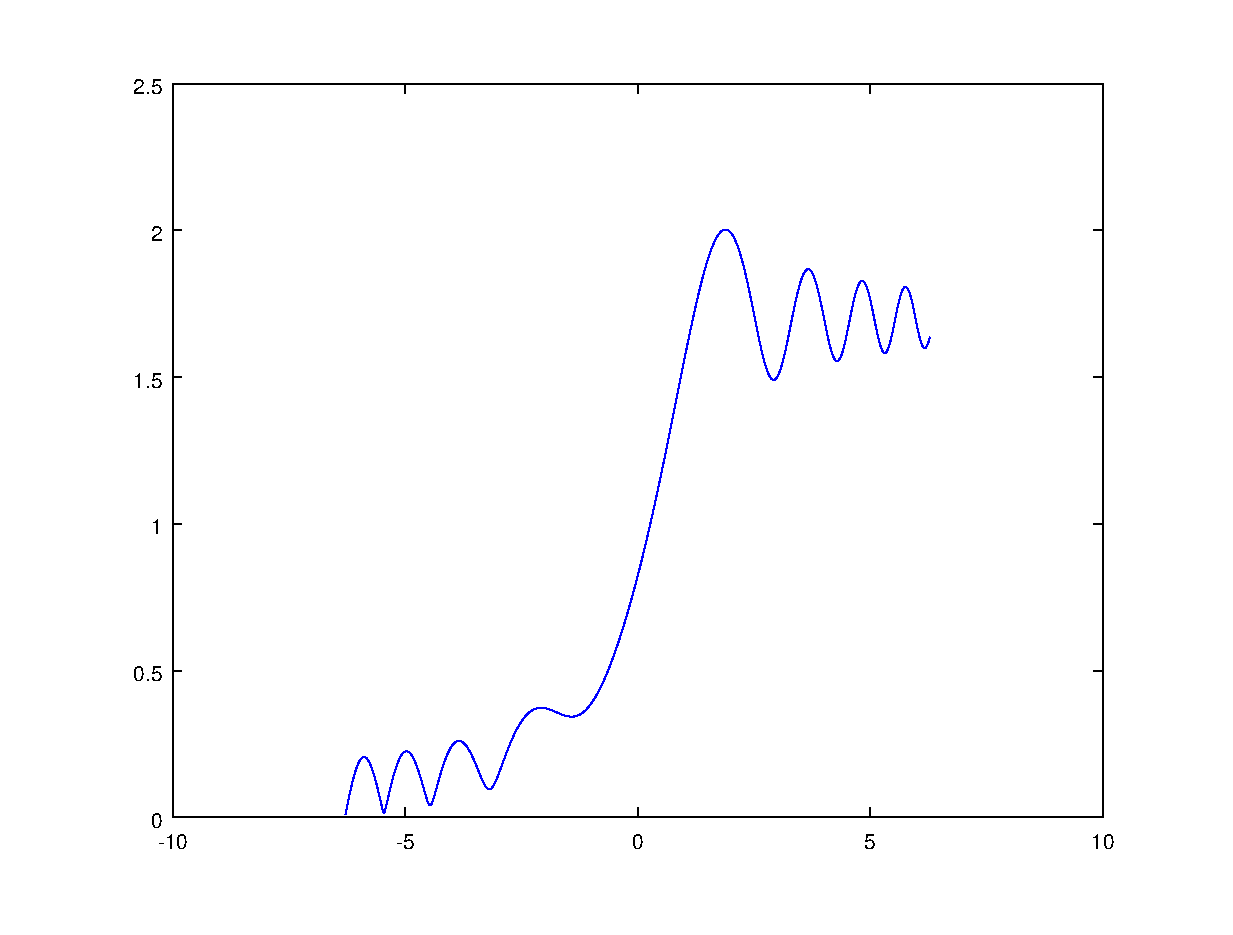
\includegraphics[width=0.8\textwidth]{4.eps}
\subsection{Let t=[0:0.01:2*pi], x=exp(j*t), and B=[1 3; 2 4].  Answer the following questions.}  

\subsubsection{Plot the trajectory of x on a 2-dimensional plane.  Use plot(real(x),  imag(x), ‘--r*’).} 

\subsubsection{Find the matrix cx whose first row is real(x) and whose second row is imag(x). cx is the set of points } 

\subsubsection{Compute z=B*cx.  z is the linear transformation of x by matrix B.  And plot z using plot(z(1,:), z(2,:)) over the plot (a).} 
\begin{lstlisting}
t = [0:0.01:2*pi];
x = exp(j * t);
B = [1 3;2 4]
plot(real(x), imag(x), '-r*')
cx = [real(x); imag(x)];
z = B * cx;
hold on
plot(z(1,:), z(2,:))
\end{lstlisting}
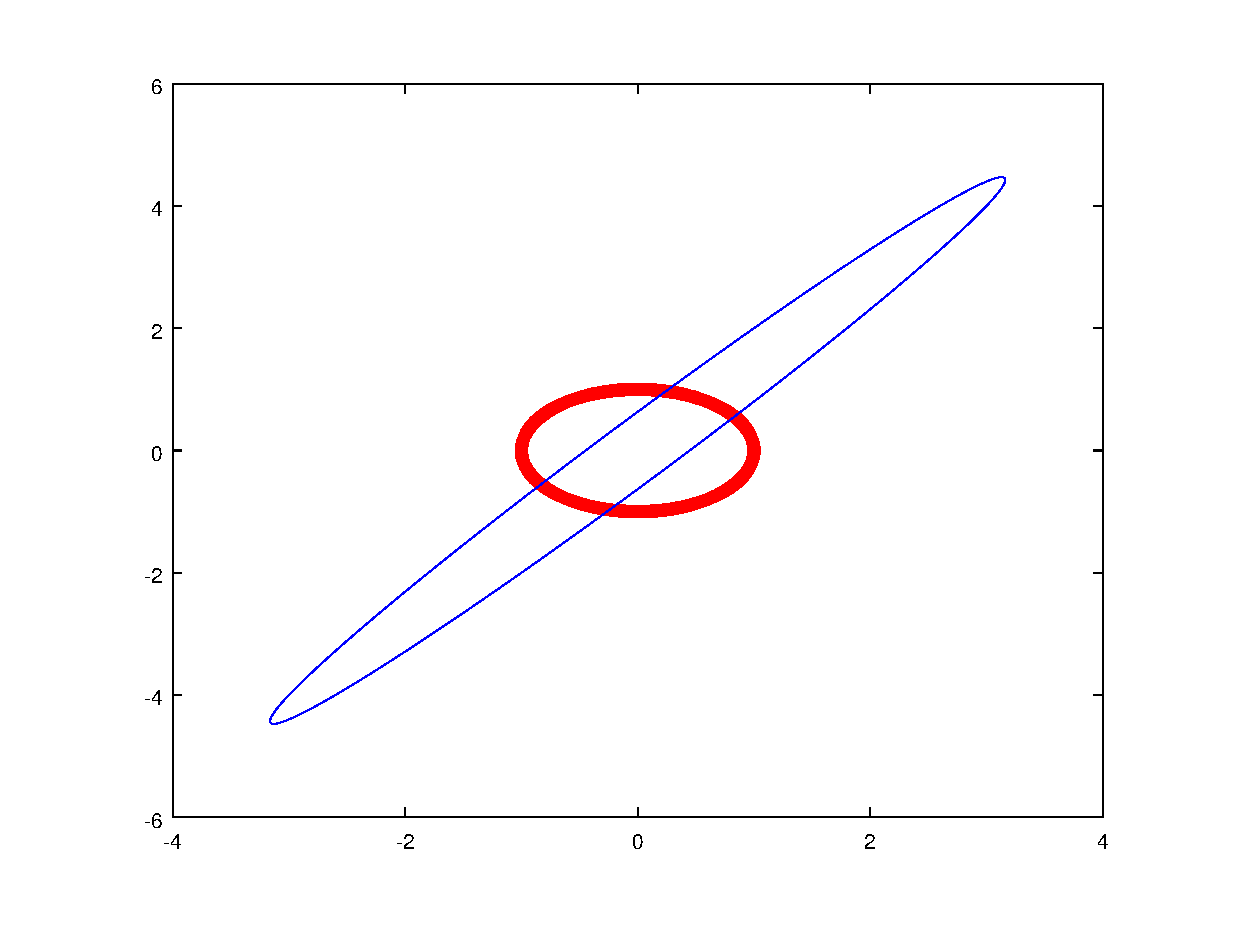
\includegraphics[width=0.8\textwidth]{5.eps}
\end{document}
